\section{Non-crossing 2-partitions}

\begin{definition}[Non-crossing 2-partition]
    A \emph{non-crossing 2-partition} of a \emph{totally
    ordered} set $E$ is a pair $(P, \sigma)$
    where :\\
    \begin{itemize*}
        \item $P$ is a non-crossing partition of $E$\\
        \item $\sigma$ is a permutation of the elements of $E$\\
        \item For each \emph{sorted} block
            $B_i = \{b_1, \ldots, b_k\} \in P$, we have
            $\sigma (b_i) < \ldots < \sigma (b_k)$\\\\
    \end{itemize*}
\end{definition}

We denote by $\mathcal{NC}^2_n$ the set of non-crossing
2-partitions of $[n]$.
$$\mathcal{NC}^2 = \bigcup_{n > 0}{\mathcal{NC}^2_n}$$.

\begin{example}[$\mathcal{NC}^2_6$]
    \begin{itemize*}
            \subitem $P = \{\{1, 6\}, \{2, 3, 5\}, \{4\}\}$
            \subitem $\sigma = 413265$ \\
            \subitem $\hspace{36mm} \rho = \{\{1, 3, 6\}, \{2\}, \{4, 5\}\}$
    \end{itemize*}    
\end{example}

\begin{theorem}[Edelman, 1979]
    Let $nc^2_n$ be the cardinal of $\mathcal{NC}^2_n$.
    We have $$nc^2_n = (n + 1)^{n-1}$$
\end{theorem}

\begin{example}[$n = 1, 2, 3$]
    ~\\
    \begin{itemize}
            \item $n = 1$ \  $:$ \  $nc^2_1 = 1$
            \subitem $\{\{1\}\}$ \hspace{1cm} $1$
                \hspace{1cm} $\rho = P$
            \item $n = 2$ \  $:$ \  $nc^2_2 = 3$
            \subitem $\{\{1\}, \{2\}\}$ \hspace{1cm} $12$
                \hspace{1cm} $\rho = P$
            \subitem $\{\{1\}, \{2\}\}$ \hspace{1cm} $21$
                \hspace{1cm} $\rho = P$
            \subitem $\{\{1, 2\}\}$ \hspace{14mm} $12$
                \hspace{1cm} $\rho = P$
            \item $n = 3$ \  $:$ \  $nc^2_3 = 16$
            \subitem $\{\{1\}, \{2\}, \{3\}\}$ \hspace{1cm}
                $123$ \hspace{1cm} $\rho = P$
            \subitem $\{\{1\}, \{2\}, \{3\}\}$ \hspace{1cm}
                $132$ \hspace{1cm} $\rho = P$
            \subitem $\{\{1\}, \{2\}, \{3\}\}$ \hspace{1cm}
                $213$ \hspace{1cm} $\rho = P$
            \subitem $\{\{1\}, \{2\}, \{3\}\}$ \hspace{1cm}
                $231$ \hspace{1cm} $\rho = P$
            \subitem $\{\{1\}, \{2\}, \{3\}\}$ \hspace{1cm}
                $312$ \hspace{1cm} $\rho = P$
            \subitem $\{\{1\}, \{2\}, \{3\}\}$ \hspace{1cm}
                $321$ \hspace{1cm} $\rho = P$       
            \subitem $\{\{1, 2\}, \{3\}\}$ \hspace{14mm}
                $123$ \hspace{1cm} $\rho = P$
            \subitem $\{\{1, 2\}, \{3\}\}$ \hspace{14mm}
                $132$ \hspace{1cm} $\rho = \{\{1, 3\}, \{2\}\}$
            \subitem $\{\{1, 2\}, \{3\}\}$ \hspace{14mm}
                $231$ \hspace{1cm} $\rho = \{\{1\}, \{2, 3\}\}$
            \subitem $\{\{1\}, \{2, 3\}\}$ \hspace{14mm}
                $123$ \hspace{1cm} $\rho = P$
            \subitem $\{\{1\}, \{2, 3\}\}$ \hspace{14mm}
                $213$ \hspace{1cm} $\rho = \{\{1, 3\}, \{2\}\}$
            \subitem $\{\{1\}, \{2, 3\}\}$ \hspace{14mm}
                $312$ \hspace{1cm} $\rho = \{\{1, 2\}, \{3\}\}$
            \subitem $\{\{1, 3\}, \{2\}\}$ \hspace{14mm}
                $123$ \hspace{1cm} $\rho = P$
            \subitem $\{\{1, 3\}, \{2\}\}$ \hspace{14mm}
                $132$ \hspace{1cm} $\rho = \{\{1, 2\}, \{3\}\}$
            \subitem $\{\{1, 3\}, \{2\}\}$ \hspace{14mm}
                $213$ \hspace{1cm} $\rho = \{\{1\}, \{2, 3\}\}$  
            \subitem $\{\{1, 2, 3\}\}$ \hspace{18mm}
                $123$ \hspace{1cm} $\rho = P$\\
    \end{itemize}
\end{example}

\begin{prop}
    This means we can create a \emph{bijection} between
    $\mathcal{PF}_n$ and $\mathcal{NC}^2_n$.
\end{prop}

\begin{proof}
    ~\\
\begin{itemize}
    \item $\mathcal{PF}_n \to \mathcal{NC}^2_n$ :
    Let $f = (a_1, \ldots, a_n) \in \mathcal{PF}_n$
    be our parking function.
    For $i \in \{1, \ldots, n\}$, we define :
        \subitem $l_i$ : the number of occurences of $i$ in $f$. 
        \subitem $im_i$ : $\{j\ |\ a_j = i\}$\\
    The corresponding non-crossing partition will
    have the following constraints :
        \subitem For each $i \in \{1, \ldots, n\}$, if $l_i > 0$,
        then there is a block $B_{[i]}$ of length
        \subitem $l_i$ with minimum element $i$.
        \subitem $\sigma (B_{[i]}) = im_i$\\
    There is a unique set partition
    $\displaystyle P = \bigcup_{i}{B}_{[i]}$ of $[n]$
    and a unique permutation $\sigma$ respecting these
    conditions such that $(P, \sigma) \in \mathcal{NC}^2_n$ :
    for each minimum $i$ in \emph{decreasing order}, add
    the $n_i$ first free elements of
    $[i+1, i+2, \ldots, n, 1, \ldots, i-1]$ to $B_i$.
    $\sigma$ is then trivially obtained by the second
    constraint. 
    \item $\mathcal{NC}^2_n \to \mathcal{PF}_n$ :
    Let $(P, \sigma)$ with $P = \{B_1, \ldots, B_l\}$ be our
    non-crossing 2-partition.
    For each block $B_i = \{b_1, \ldots, b_k\} \in P$ :
    \subitem $m_i = min (B_i) = b_1$
    \subitem $pos_i = \sigma (B_i)$
    \subitem For each $j \in pos_i$, we define $a_j = m_i$\\
    The corresponding parking function is $(a_1, \ldots, a_n)$.
\end{itemize}
\end{proof}

\begin{example}[$n = 8$]
    \begin{align*}
        &P = \{\{1, 2, 5\}, \{3, 4\}, \{6, 8\}, \{7\}\}\\
        &\sigma = 36187245\\
        &f = (3, 6, 1, 7, 6, 1, 1, 3)\\
    \end{align*}
\end{example}

Following the path of the classical primitive case, we recall
the cover relation defined in \cite{ref9} in order to deduce
a poset for $\mathcal{PF}_n$.

\subsection{The non-crossing 2-partitions poset}

\begin{definition}[$\succ^2$]
    We say that $(P, \sigma)$ covers $(Q, \tau)$, written
    ($P, \sigma) \succ^2 (Q, \tau)$,
    if $\exists B_i, B_j \in P$ such that\\
    \begin{itemize*}
        \item $Q = P - \{B_i, B_j\} \cup \{B_i \cup B_j\}$\\
        \item $l \neq i, j \and b \in B_l \rightarrow
            \tau (b) = \sigma (b)$\\
        \item Let $B_i \cup B_j = \{b_1, \ldots, b_k\}$ :\\
            \subitem $\tau (B_i \cup B_j) = \sigma (B_i \cup B_j)$\\
            \subitem $\tau (b_1) < \ldots < \tau (b_k)$
    \end{itemize*}    
\end{definition}

\begin{example}
    ~\\
    \begin{itemize*}
        \item $P = \{\{1, 6\}, \{2, 3\}, \{4\}, \{5\}\}$\\
        \item $\sigma = 236154$\\
        \item $Q = \{\{1, 6\}, \{2, 3, 5\}, \{4\}\}$\\
        \item $\tau = 235164$\\
        \item $(P, \sigma) \succ^2 (Q, \tau)$\\
        \item $(P, \sigma) \not \succ^2 (Q, \sigma)$,
        because  $\sigma (\{2, 3, 5\}) = \{3, 6, 5\}$ is
        \emph{not} ordered. 
    \end{itemize*}
\end{example}

\begin{prop}
    This covering relation defines the \emph{poset} of
    $\mathcal{NC}^2_n$.
\end{prop}

\begin{rem}
    The bottom element of this poset is 
    $(\{\{1, \ldots, n\}\}, 12 \ldots n)$, and the top
    elements are $\{(\{\{1\}, \ldots, \{n\}\}, \sigma)\ 
    |\ \sigma \in \mathfrak{S}_n\}$.
\end{rem}

\begin{example}[The poset of $\mathcal{NC}^2_3$]
    ~\\
    To shorten labels, we represent
    $(\{\{1, 3\}, \{2\}\}, 213)$ by \\
    \begin{center}
        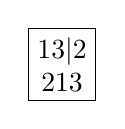
\begin{tikzpicture}
            \node (0) at (0,0) [align = center]
            [rectangle, draw]{$13|2$\\$213$};
        \end{tikzpicture}
    \end{center}

    \begin{center}
        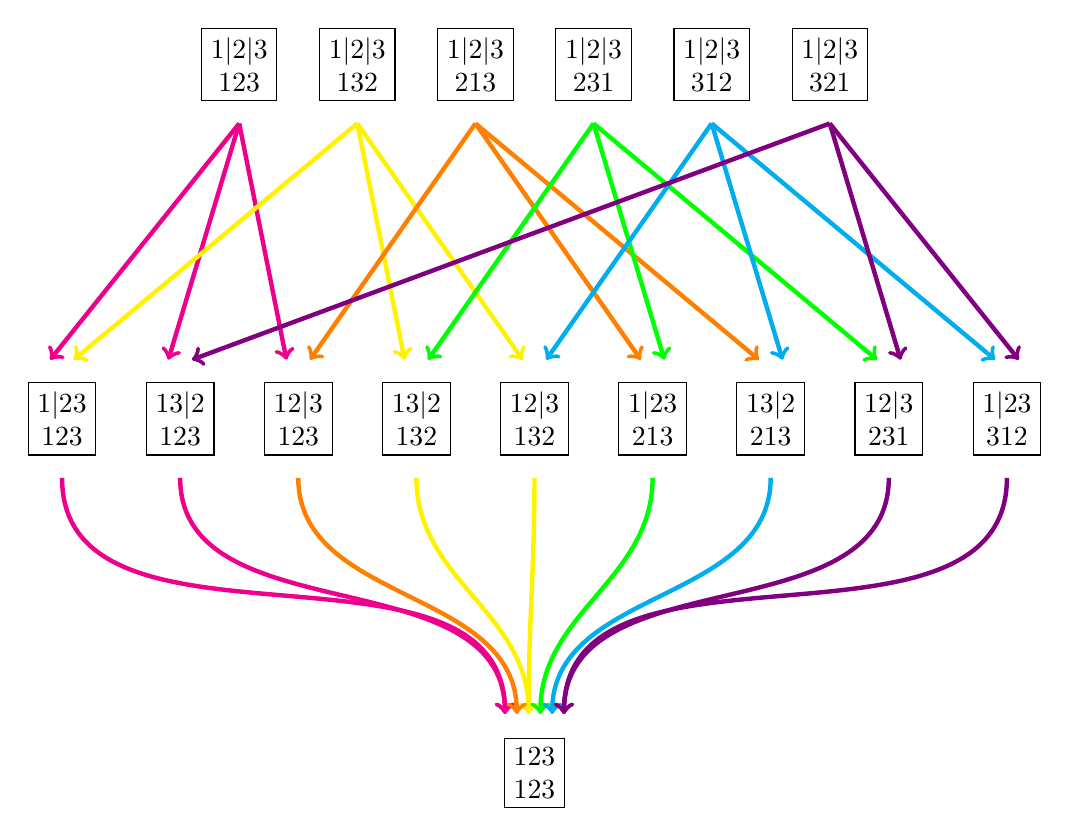
\begin{tikzpicture}[scale = 0.75]
    \node (0)  at (0,0) [align = center]
    [rectangle, draw]
        {$123$\\$123$};
    \node (1)  at (-8,6)[align = center]
    [rectangle, draw]
        {$1|23$\\$123$};
    \node (2)  at (-6,6) [align = center]
    [rectangle, draw]
        {$13|2$\\$123$};
    \node (3)  at (-4,6) [align = center]
    [rectangle, draw]
        {$12|3$\\$123$};
    \node (4)  at (-2,6) [align = center]
    [rectangle, draw]
        {$13|2$\\$132$};
    \node (5)  at (0,6) [align = center]
    [rectangle, draw]
        {$12|3$\\$132$};
    \node (6)  at (2,6) [align = center]
    [rectangle, draw]
        {$1|23$\\$213$};
    \node (7)  at (4,6) [align = center]
    [rectangle, draw]
        {$13|2$\\$213$};
    \node (8)  at (6,6) [align = center]
    [rectangle, draw]
        {$12|3$\\$231$};
    \node (9)  at (8,6) [align = center]
    [rectangle, draw]
        {$1|23$\\$312$};
    \node (10) at (-5,12) [align = center]
    [rectangle, draw]
        {$1|2|3$\\$123$};
    \node (11) at (-3,12) [align = center]
    [rectangle, draw]
        {$1|2|3$\\$132$};
    \node (12) at (-1,12) [align = center]
    [rectangle, draw]
        {$1|2|3$\\$213$};
    \node (13) at (1,12) [align = center]
    [rectangle, draw]
        {$1|2|3$\\$231$};
    \node (14) at (3,12) [align = center]
    [rectangle, draw]
        {$1|2|3$\\$312$};
    \node (15) at (5,12) [align = center]
    [rectangle, draw]
        {$1|2|3$\\$321$};

    \draw [->][color=magenta, ultra thick]
        (-5,11) to (-8.2,7);
    \draw [->][color=magenta, ultra thick]
        (-5,11) to (-6.2, 7); 
    \draw [->][color=magenta, ultra thick]
        (-5,11) to (-4.2,7);
    \draw [->][out=-90,in=90, ultra thick] 
        [color=magenta](-8,5) to (-0.5,1);
    \draw [->][out=-90,in=90, ultra thick] 
        [color=magenta](-6,5) to (-0.5,1);

    \draw [->][color=yellow, ultra thick]
        (-3,11) to (-7.8,7);
    \draw [->][color=yellow, ultra thick]
        (-3,11) to (-2.2,7);
    \draw [->][color=yellow, ultra thick]
        (-3,11) to (-0.2, 7);
    \draw [->][out=-90,in=90, ultra thick] 
        [color=yellow](-2,5) to (-0.1,1);
    \draw [->][out=-90,in=90, ultra thick] 
        [color=yellow](0,5) to (-0.1,1);
    
    \draw [->][color=orange, ultra thick]
        (-1,11) to (1.8,7);
    \draw [->][color=orange, ultra thick]
        (-1,11) to (3.8,7);
    \draw [->][color=orange, ultra thick]
        (-1,11) to (-3.8,7);
    \draw [->][out=-90,in=90, ultra thick] 
        [color=orange](-4,5) to (-0.3,1);

    \draw [->][color=green, ultra thick]
        (1,11) to (2.2,7);
    \draw [->][color=green, ultra thick]
        (1,11) to (-1.8,7);
    \draw [->][color=green, ultra thick]
        (1,11) to (5.8,7);
    \draw [->][out=-90,in=90, ultra thick] 
        [color=green](2,5) to (0.1,1);

    \draw [->][color=cyan, ultra thick]
        (3,11) to (7.8,7);
    \draw [->][color=cyan, ultra thick]
        (3,11) to (4.2,7);
    \draw [->][color=cyan, ultra thick]
        (3,11) to (0.2,7);
    \draw [->][out=-90,in=90, ultra thick] 
        [color=cyan](4,5) to (0.3,1);

    \draw [->][color=violet, ultra thick]
        (5,11) to (8.2,7);
    \draw [->][color=violet, ultra thick]
        (5,11) to (-5.8,7);
    \draw [->][color=violet, ultra thick]
        (5,11) to (6.2,7);
    \draw [->][out=-90,in=90, ultra thick] 
        [color=violet](6,5) to (0.5,1);
    \draw [->][out=-90,in=90, ultra thick] 
        [color=violet](8,5) to (0.5,1);
    
\end{tikzpicture}
        ~\\
        There are $4^2 = 16$ elements in this poset.
    \end{center}
\end{example}

We can now define a poset for $\mathcal{PF}_n$, in which
the \emph{height} of any parking function will be defined
by its \emph{rank}.

\subsection{The parking functions poset}

\begin{definition}[Rank]
    Given $f = (a_1, \ldots, a_n) \in \mathcal{PF}_n$, let
    $$b_i =
    \begin{cases}
        1 \text{ if } \exists j\ |\ a_j = i\\
        0 \text{ otherwise}
    \end{cases} $$
    We define the \emph{rank} of $f$, noted $rk(f)$, as
    $$\sum_{1 \leq i \leq n}{b_i}$$
\end{definition}

\begin{example}
    \begin{align*}
        &rk((1, 5, 4, 2, 3, 3, 1)) = 5\\
        &rk((4, 7, 1, 1, 3, 2 ,2, 8)) = 6\\
    \end{align*}
\end{example}

\begin{definition}[$\succ_{pf}$]
    Since $\mathcal{PF}_n$ and $\mathcal{NC}^2_n$ are
    in bijection, we can define a \emph{covering relation}
    $\succ_{pf}$ for $\mathcal{PF}_n$ as follows :\\
    $f \in \mathcal{PF}_n \succ_{pf} g \in \mathcal{PF}_n$
    if and only if :    
    \begin{itemize}
        \item $(P,\sigma)$ is the non-crossing 2-partition
        associated to $f$
        \item $(Q, \tau)$ is the non-crossing 2-partition
        associated to $g$
        \item $(P, \sigma) \succ^2 (Q, \tau)$
    \end{itemize}
\end{definition}

\begin{example}
    ~\\
    \begin{itemize*}
        \item $P = \{\{1, 6\}, \{2, 3\}, \{4\}, \{5\}\}$\\
        \item $\sigma = 236154$\\
        \item $Q = \{\{1, 6\}, \{2, 3, 5\}, \{4\}\}$\\
        \item $\tau = 235164$\\
        \item $f = (4, 1, 2, 1, 5, 2) \succ_{pf}
            g = (4, 1, 2, 1, 2, 2)$\\
    \end{itemize*}
\end{example}

\begin{rem}
    If $f \succ_{pf} g$, then $rk(f) = rk(g) + 1$, and
    there exists $i$ and $j$ such that :
    \begin{itemize}
        \item $i < j$
        \item There is at least $1$ occurence of $i$ in $f$
        \item There is at least $1$ occurence of $j$ in $f$
        $$b_k =
            \begin{cases}
                i \text{ if } a_k = j\\
                a_k \text{ otherwise}\\
            \end{cases}$$
    \end{itemize}
\end{rem}

\begin{prop}
    This covering relation defines the \emph{poset}
    of $\mathcal{PF}_n$.
\end{prop}

\begin{rem}
    The bottom element of this poset is
    $(\underbrace{1, \ldots, 1}_{n})$,
    and the top elements are the \emph{permutations} of
    $\{1, \ldots, n\}$.
\end{rem}

\begin{example}[The poset of $\mathcal{PF}_3$]
    \begin{center}
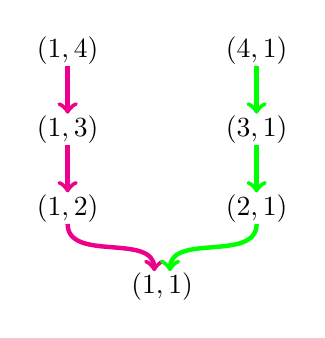
\begin{tikzpicture}[scale = 0.2]
    \node at (0,0) {$(1,1)$};

    \node at (-6,5) {$(1,2)$};
    \node at (6,5)  {$(2,1)$};

    \node at (-6,10) {$(1,3)$};
    \node at (6,10)  {$(3,1)$};

    \node at (-6,15) {$(1,4)$};
    \node at (6,15)  {$(4,1)$};

    \draw [->][color=magenta, ultra thick]
        (-6,14) to (-6,11);
    \draw [->][color=magenta, ultra thick]
        (-6,9) to (-6,6);
    \draw [->][out=-90,in=90, ultra thick] 
        [color=magenta](-6,4) to (-0.5,1);

    \draw [->][color=green, ultra thick]
        (6,14) to (6,11);
    \draw [->][color=green, ultra thick]
        (6,9) to (6,6);
    \draw [->][out=-90,in=90, ultra thick] 
        [color=green](6,4) to (0.5,1);

\end{tikzpicture}
\end{center}
\end{example}

While non-crossing (2-)partitions are frequently used to
define a poset for (primitive) parking functions, it is
rather unpractical that using a bijection to define the
cover relation is necessary.\\
Thereby, the following section will present our tentative
at finding a more direct definition for the cover relation
of $\mathcal{PF}_n$ and  $\mathcal{PF'}_n$, this time using
a bijection with (decorated) Dyck Paths.
A main benefit of this solution is that we define a cover
relation for both structures, and the poset of one can be
obtained by applying the given bijection to the poset of the
other.\\
Furthermore, the two main results of this article -- Theorem 8
and the corresponding Conjecture for the classical case --
rise from the number of intervals in those posets.   